\section{Materiais e Métodos}

%%%%%%%%%%%%%%%%%%%%%%%%%%%%%%%%%%%%%%%%%%%
%% VISÃO GERAL
%%%%%%%%%%%%%%%%%%%%%%%%%%%%%%%%%%%%%%%%%%%
\subsection{Visão Geral}

Pelo fluxograma da figura \ref{fig:fluxogram}, vemos que a primeira etapa no desenvolvimento da Rede Neural Convolucional é a aquisição e o pré-processamento dos dados. A criação da estrutura (sequência de camadas da rede neural) e o ajuste dos hiperparâmetros, também chamdo de \emph{fine tunning}, vem em seguida. É o treimento que une a primeira e a segunda etapa, pois é nele que os dados pré-processados são inseridos na estrutura modelada. Logo em seguida, é feita uma validação da rede treinada. É o desempenho da modelagem anterior que dá o \emph{feedback} das modificações necessárias para a próxima versão da estrutura. O desenvolvimento do modelo termina quando é atingida uma boa acurácia de predição.

\begin{figure}[h!]
  \centering
  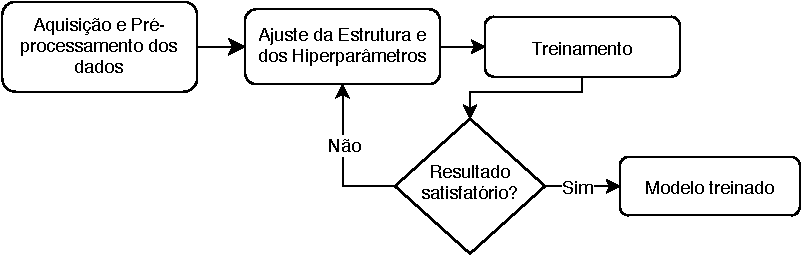
\includegraphics[width=\textwidth]{figures/dl_diagram.pdf}
  \caption{Fluxograma do desenvolvimento do modelo.}
  \label{fig:fluxogram}
\end{figure}

%%%%%%%%%%%%%%%%%%%%%%%%%%%%%%%%%%%%%%%%%%%%%
%% AQUISIÇÃO DOS DADOS
%%%%%%%%%%%%%%%%%%%%%%%%%%%%%%%%%%%%%%%%%%%%%
\subsection{Aquisição dos dados}

Dados de treinamento são elementos fundamentais para o treinamento supervisionado de uma Rede Neural Artificial. Para treinar uma rede que aprenda a classificar galáxias de acordo com suas imagens é necessário fazê-la aprender formas e padrões das galáxias. Para isso, é necessário separar uma grande amostra de imagens de galáxias já classificadas por humanos.

A fonte dos dados são GalaxyZoo, que contém as classificações morfológicas, e os levantamentos SDSS e S-PLUS, que possuem as imagens das galáxias. A associação dos dados entre estas duas fontes são feitas pelas coordenadas do objeto no espaço.

As imagens do SDSS foram obtidas usando a \emph{API}\footnote{API: \emph{Application Programming Interface}. É uma interface de comicação entre sistemas.} do SDSS\footnote{Documentação da API: http://skyserver.sdss.org/dr16/en/help/docs/api.aspx.}. Já as imagens do S-PLUS foram obtidas pela contribuição dos algorítmos\footnote{Página do repositório: https://github.com/lucatelli/splus-tools.} de Geferson Lucatelli. A figura \ref{fig:galaxy_grid} é um exemplo das imagens RGB do SDSS.

\begin{figure}[h!]
  \centering
  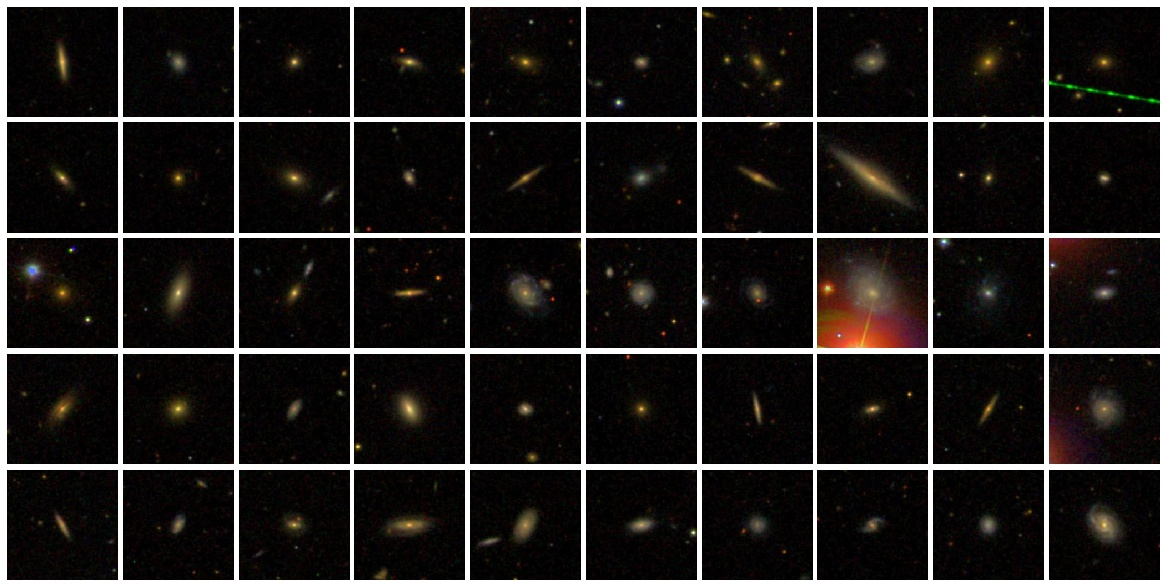
\includegraphics[width=\textwidth]{figures/galaxy_grid.jpg}
  \caption{Amostra com cinquenta imagens de galáxias (escala reduzida).}
  \label{fig:galaxy_grid}
\end{figure}

%%%%%%%%%%%%%%%%%%%%%%%%%%%%%%%%%%%%%%%%%%%
%% DIVISÃO DO CONJUNTO DE DADOS
%%%%%%%%%%%%%%%%%%%%%%%%%%%%%%%%%%%%%%%%%%%
\subsection{Divisão do conjunto de dados}

O conjunto de dados é dividido em três subconjuntos: treinamento, validação e teste. Os dois primeiros são usados durante o treinamento, portanto, são com estes dados que a rede irá aprender, e o subjunto de teste é usado após o treinameto para verificar a generalidade da rede, ou seja, determinar se a rede consegue classificar uma imagem não vista antes.

Todos os modelos usam o mesmo conjunto de dados, para garantir que o desempenho de classificação do modelo não foi afetado pelos dados. Embora a fonte de dados seja diferente entre os modelos, imagens RGB do SDSS para alguns e fluxo de fótons do S-PLUS para outros, ambos os conjunto de dados tem exatamente os mesmos objetos em cada um dos subconjuntos.

Para cada subconjunto, é separada uma quantidade de amostras relativa à quantidade total de cada classe: 72\% para o treino, 18\% para a validação e 10\% para o teste. A tabela \ref{tab:img_qtd} mostra a quantidade de imagens para cada um dos subconjuntos conforme a classe.

\begin{table}[h!]
  \centering

  \caption{Quantidade de amostras de imagens de galáxias por classe.}
  \label{tab:img_qtd}

  \renewcommand{\arraystretch}{1.6}
  \begin{tabular}{ccccc}
    \toprule
    \thead{Classe} & \thead{Treinamento                       \\(72\%)} & \thead{Validação\\(18\%)} & \thead{Teste\\(10\%)} & \thead{Total} \\
    \midrule
    E              & 4.504              & 1.126 & 625 & 6.255 \\
    S              & 1.370              & 342   & 190 & 1.902 \\
    Total          & 5.874              & 1.468 & 815 & 8.157 \\
    \bottomrule
  \end{tabular}
\end{table}

Como as classes não são balanceadas, ou seja, há uma quantidade de amostra muito maior em uma classe que em outra, pesos foram utilizados em cada classe. O peso $w_i$ da i-ésima classe tem o valor dado pela equação \ref{eq:pesos}.
\begin{equation}
  w_i = \frac{Q}{N \times C_i}
  \label{eq:pesos}
\end{equation}
onde, $Q$ é a quantidade total de amostras, $N$ é o número de classes e $C_i$ é o número de amostras da i-ésima classe.

%%%%%%%%%%%%%%%%%%%%%%%%%%%%%%%%%%%%%%%%%%%%%%
%% PRÉ-PRECESSAMENTO DOS DADOS
%%%%%%%%%%%%%%%%%%%%%%%%%%%%%%%%%%%%%%%%%%%%%%
\subsection{Pré-processamento dos dados}

O pré-processamento é a preparação das imagens para serem usadas pelo modelo, ou seja, é a transformação dos dados brutos em dados reconhecíveis pela rede. Isso envolve representar as imagens por  matrizes multidimensionais, onde cada elemento da matriz representa um pixel da imagem, e aplicar algumas transformações, especificadas a seguir. Todos os modelos usam imagens do tamanho 64x64 pixels.

Como as imagens do SDSS usadas estão no sistema de cor RGB, o tensor de entrada da rede terá dimensão (64, 64, 3). As primeiras duas dimensões são referentes ao comprimento e largura da imagem e a terceira aos três canais de cores RGB.

Já os dados do S-PLUS não foram processados e para o padrão de cor RGB e, portanto, informações de todas as 12 bandas fotométricas são usadas. Para que seja possível usar uma rede pré-treinada, a entrada é dividida em 4 tensores (64, 64, 3).

Todas as imagens são reescaladas para o intervalo [0, 1], dividindo cada elemento pelo valor máximo da imagem. Além disso, para as imagens do S-PLUS, a mediana da imagem é subtraída de cada pixel. Já que a mediana da imagem é uma aproximação do valor do céu.

%%%%%%%%%%%%%%%%%%%%%%%%%%%%%%%%%%%%%%%%%%%%%%
%% MODELAGEM DA REDE NEURAL ARTIFICIAL
%%%%%%%%%%%%%%%%%%%%%%%%%%%%%%%%%%%%%%%%%%%%%%
\subsection{Modelagem e Ajuste dos Hiperparâmetros}

A rede neural artificial foi programada em Python e a biblioteca Keras\footnote{Uma API de alto nível criada para modelagem e treinamento de redes neurais que, neste projeto, roda sobre o TensorFlow. Tem foco em permitir experimentação rápida.} foi usada para criar e treinar o modelo.

A modelagem é a criação de uma estrutura. Isto inclui: a escolha da quantidade de camadas, a definição do tipo de cada camada e a especificação da sequência em que as camadas aparecerão. Já os hiperparâmetros são os atributos de cada camada ou do modelo em geral. Alguns exemplos de hiperparâmetros são: a taxa de aprendizagem\footnote{A velocidade com que a rede neural aprende os padrões.} (\emph{learning rate}), a quantidade de unidades\footnote{A quantidade de neurônios artificais.} de cada camada e a taxa (\emph{rate}) das camadas \emph{dropout}. Estes ajustes são feitos empiricamente e reajustados de acordo com o resultado obtido após o treinamento, como visto na figura \ref{fig:fluxogram}.

\pagebreak
\begin{figure}[ht!]
  \centering
  \begin{minipage}[t]{.47\textwidth}
    \centering
    \tikzset{
>=stealth',
  punktchain/.style={
    rectangle, 
    rounded corners, 
    % fill=black!10,
    draw=black, thick,
    text width=8em, 
    minimum height=2em, 
    text centered, 
    on chain},
  line/.style={draw, thick, <-},
  element/.style={
    tape,
    top color=white,
    bottom color=blue!50!black!60!,
    minimum width=8em,
    draw=blue!40!black!90, very thick,
    text width=8em, 
    minimum height=2em, 
    text centered, 
    on chain},
  every join/.style={->, thick, shorten >=1pt},
}

\begin{tikzpicture}
    [node distance=.5cm,
    start chain=going below,]
    \node[punktchain, join] (input) {\small Input};
    \node[punktchain, join] (conv_1) {\small Conv2D};
    \node[punktchain, join] (maxpool_1) {\small MaxPooling2D};
    \node[punktchain, join] (conv_2) {\small Conv2D};
    \node[punktchain, join] (maxpool_2) {\small MaxPooling2D};
    \node[punktchain, join] (conv_3) {\small Conv2D};
    \node[punktchain, join] (maxpool_3) {\small MaxPooling2D};
    \node[punktchain, join] (conv_4) {\small Conv2D};
    \node[punktchain, join] (maxpool_4) {\small MaxPooling2D};
    \node[punktchain, join] (flatten) {\small Flatten};
    \node[punktchain, join] (dense_1) {\small Dense};
    \node[punktchain, join] (dense_2) {\small Dense};
\end{tikzpicture}
    \captionof{figure}{\textbf{Modelo 1} -- Camadas convolucionais intercaladas com camadas \emph{pooling}.}
    \label{fig:conv_model}
  \end{minipage}%
  \hfill%
  \begin{minipage}[t]{.47\textwidth}
    \centering
    \tikzset{
  >=stealth',
  punktchain/.style={
      rectangle,
      rounded corners,
      draw=black, thick,
      text width=8em,
      minimum height=2em,
      text centered,
      on chain},
  line/.style={draw, thick, <-},
  every join/.style={->, thick, shorten >=1pt},
}

\begin{tikzpicture}
  [node distance=.5cm,
    start chain=going below,]
  \node[punktchain, join] (input) {\small Input};
  \node[punktchain, join] (vgg16) {\small VGG16};
  \node[punktchain, join] (flatten) {\small Flatten};
  \node[punktchain, join] (dense_1) {\small Dense};
  \node[punktchain, join] (dropout_1) {\small Dropout};
  \node[punktchain, join] (dense_2) {\small Dense};
  \node[punktchain, join] (dropout_2) {\small Dropout};
  \node[punktchain, join] (dense_3) {\small Dense};
  \node[punktchain, join] (dropout_3) {\small Dropout};
  % \node[punktchain, join] (dense_4) {\small Dense};
  % \node[punktchain, join] (dropout_4) {\small Dropout};
  \node[punktchain, join] (dense_5) {\small Dense};
\end{tikzpicture}
    \captionof{figure}{\textbf{Modelo 2} -- Rede pré-treinada ligada à uma rede densa com \emph{dropout}.}
    \label{fig:pretrained_model}
  \end{minipage}
\end{figure}
\pagebreak
\begin{figure}[h!]
  \centering
  \begin{tikzpicture}
  \tikzstyle{basenode} = [rectangle, rounded corners, minimum width=3cm, minimum height=1cm,text centered, draw=black, align=center]
  \tikzstyle{arrow} = [thick,->,>=stealth]

  \node (inp1) [basenode]
  {{\bf Input 1}\\{\small (64, 64, 3)}\\{\footnotesize F378, F395, F410}};
  \node (inp2) [basenode, right of=inp1, xshift=2.5cm]
  {{\bf Input 2}\\{\small (64, 64, 3)}\\{\footnotesize F430, F515, F660}};
  \node (inp3) [basenode, right of=inp2, xshift=2.5cm]
  {{\bf Input 3}\\(64, 64, 3)\\{\footnotesize F861, G, I}};
  \node (inp4) [basenode, right of=inp3, xshift=2.5cm]
  {{\bf Input 4}\\{\small (64, 64, 3)}\\{\footnotesize R, U, Z}};
  \node (vgg1) [basenode, below of=inp1, yshift=-1cm] {{\bf VGG16}};
  \node (vgg2) [basenode, below of=inp2, yshift=-1cm] {{\bf VGG16}};
  \node (vgg3) [basenode, below of=inp3, yshift=-1cm] {{\bf VGG16}};
  \node (vgg4) [basenode, below of=inp4, yshift=-1cm] {{\bf VGG16}};
  \node (concatenate) [basenode, below of=vgg2, xshift=1.75cm, yshift=-1.5cm]
  {{\bf Concatenate}};
  \node (flatten) [basenode, below of=concatenate, yshift=-1cm] {{\bf Flatten}};
  \node (dense1) [basenode, below of=flatten, yshift=-1cm] {{\bf Dense}};
  \node (dropout1) [basenode, below of=dense1, yshift=-1cm] {{\bf Dropout}};
  \node (dense2) [basenode, below of=dropout1, yshift=-1cm] {{\bf Dense}};
  \node (out) [basenode, below of=dense2, yshift=-1cm] {{\bf Output}};

  \draw [arrow] (inp1) -- (vgg1);
  \draw [arrow] (inp2) -- (vgg2);
  \draw [arrow] (inp3) -- (vgg3);
  \draw [arrow] (inp4) -- (vgg4);
  \draw [arrow] (vgg1) -- (concatenate);
  \draw [arrow] (vgg2) -- (concatenate);
  \draw [arrow] (vgg3) -- (concatenate);
  \draw [arrow] (vgg4) -- (concatenate);
  \draw [arrow] (concatenate) -- (flatten);
  \draw [arrow] (flatten) -- (dense1);
  \draw [arrow] (dense1) -- (dropout1);
  \draw [arrow] (dropout1) -- (dense2);
  \draw [arrow] (dense2) -- (out);
\end{tikzpicture}
  \caption{\textbf{Modelo 3} -- Três tensores de entrada ligados à rede pre-treinada.}
  \label{fig:splus_model}
\end{figure}
\pagebreak

Foram criados três modelos: o primeiro, usando apenas camadas convolucionais e \emph{pooling} ligadas a uma pequena rede densa (figura \ref{fig:conv_model}) o segundo, usando uma rede pré-treinada, VGG16, ligada a uma longa rede densa com \emph{dropout} (figura \ref{fig:pretrained_model}) e o terceiro, usando quatro tensores de entrada ligados a uma rede pré-treinada (figura \ref{fig:splus_model}).

Esta rede VGG16 é treinada usando a base de dados \emph{ImageNet}\footnote{http://www.image-net.org/.}, que possui milhões de imagens de objetos do cotidaino, mas não possui objetos do espaço. A idéia é descobrir que se usar uma rede pré-treinada com milhões de imagens, mas nenhuma de galáxias, é tão relevante quanto usar uma rede treinada com apenas alguns milhares de amostras, mas todas de galáxias. Pois as redes neurais convolucionais são usadas como camada de abstração do mundo visual, ou seja, elas detectam padrões como geometrias, texturas e cores.

% Para ambos os modelos, a dimensão do tensor da entrada é (200, 200, 3). Cinco unidades na camada de saída com ativador \texttt{Softmax}. A  função de perda utilizada foi a \texttt{Categorical Crossentropy} e o otimizador foi o \texttt{RMSprop}.

% \begin{table}[h!]
%   \centering
%   \begin{tabular}{cc}
%     \toprule
%     \thead{Hiperparâmetro}          & \thead{Valor}     \\
%     \midrule
%     Ativador (Conv2D)               & ReLu              \\
%     Ativador (Dense, 1)             & ReLu              \\
%     Unidades (Conv2D)               & 32, 64, 128 e 128 \\
%     Unidades (Dense, 1)             & 512               \\
%     Dimensão do Kernel (Conv2D)     & (3, 3)            \\
%     \emph{Pool Size} (MaxPooling2D) & (2, 2)            \\
%     Taxa de aprendizagem            & $10^{-4}$         \\
%     \bottomrule
%   \end{tabular}
%   \caption{Descrição dos hiperparâmetros do Modelo 1.}
%   \label{tab:hip_model1}
% \end{table}

% \begin{table}[h!]
%   \centering
%   \begin{tabular}{cc}
%     \toprule
%     \thead{Hiperparâmetro} & \thead{Valor}        \\
%     \midrule
%     Ativador (Dense, 1-4)  & ReLu                 \\
%     Unidades (Dense, 1-4)  & 2048, 1024, 512, 256 \\
%     Taxa de \emph{dropout} & 0,5                  \\
%     Taxa de aprendizagem   & $10^{-5}$            \\
%     \bottomrule
%   \end{tabular}
%   \caption{Descrição dos hiperparâmetros do Modelo 2.}
%   \label{tab:hip_model2}
% \end{table}

% Como mostrado na figura \ref{fig:fluxogram}, diversos valores de hiperparâmetros foram ajustados empiricamente. As tabelas \ref{tab:hip_model1} e \ref{tab:hip_model2} mostram os valores dos hiperparâmetros com melhor desempenho e que são usados como exemplo nos resultados.